\documentclass[tikz]{standalone}
\usepackage{circuitikz}
\usetikzlibrary{shapes,arrows}
\begin{document}
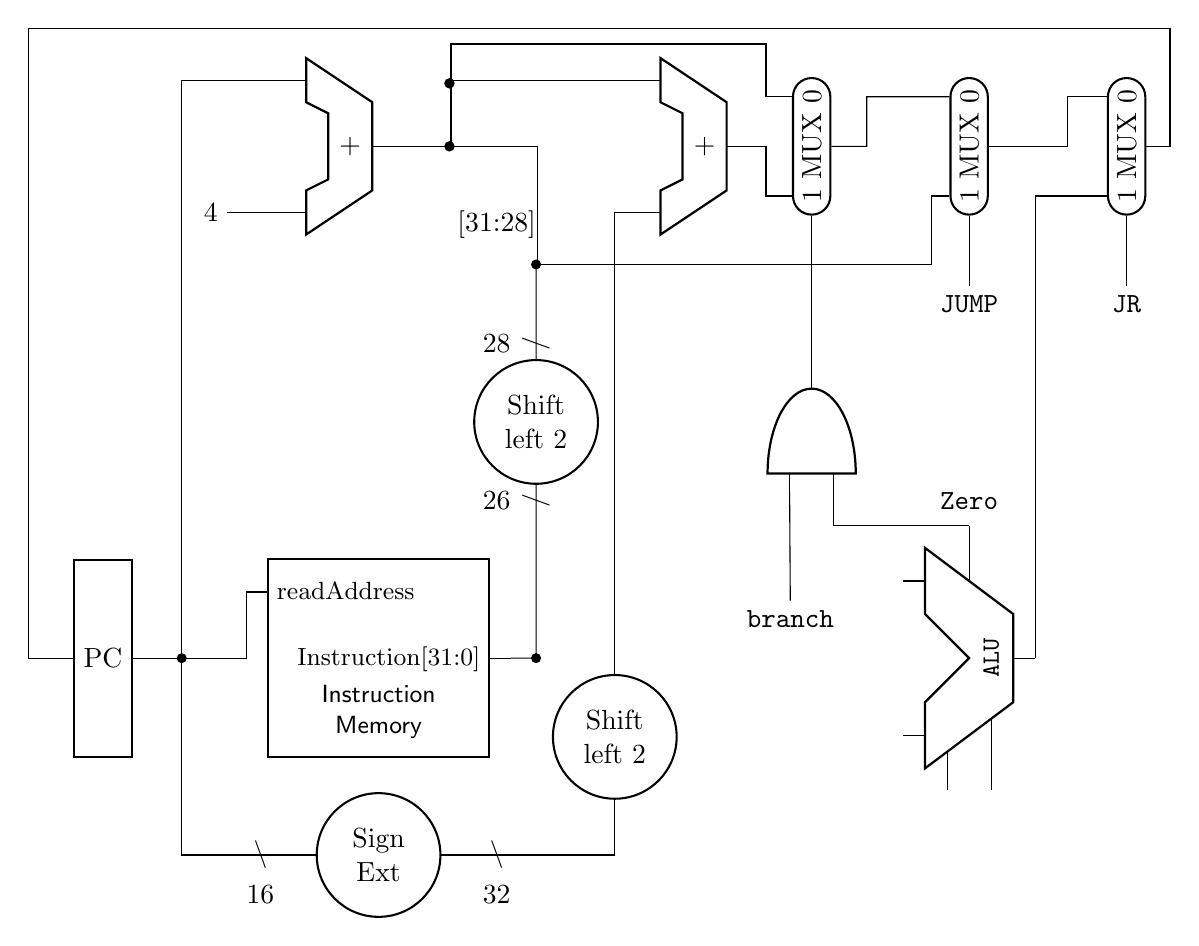
\begin{tikzpicture}
    \ctikzset{multipoles/dipchip/width=2, multipoles/flipflop/width=2}
    \tikzstyle{element} = [flipflop,text width=4.5em,text centered,font=\small\sffamily];
    \tikzstyle{mux} = [rounded rectangle,draw,rotate=90,line width=0.75pt];
    \tikzstyle{sigext} = [line width=0.75pt,draw,fill=white,text width=3em,text centered,circle];
    \node [ALU] (exALU) at (3,-1.5) {{\rotatebox{90}{\small \ttfamily ALU}}};
    %\node [element,] (PC) at (-9.5,-1.5) {PC};
    \node [draw,minimum height=2.5cm,line width=0.75pt] (PC) at (-8,-1.5) {PC};
    \node [element,flipflop def={t1=readAddress,t5=Instruction[31:0]},text height=4.5em] (Inst) at (-4.5,-1.5) {Instruction Memory};
    \draw (PC.east) to[short,-*] (-7,-1.5) -| (Inst.pin 1);
    \draw (Inst.pin 5) to[short,-*] (-2.5,-1.5) node (v8) {} to[short,-*] (-2.5,3.5) node (v9) {};

    %\node [dipchip, hide numbers, no topmark, external pins width=0,font=\small\sffamily] (Reg) at (2,-5.5) {Registers};
    %\node [right] at (Reg.bpin 1) {readReg1};
    %\node [right] at (Reg.bpin 2) {readReg2};
    %\node [right] at (Reg.bpin 3) {writeReg};
    %\node [right] at (Reg.bpin 4) {writeData};

    \node [one bit adder,external pins width=0] (oALU) at (-5,5) {+};
    \draw (-7,-1.5) node (v13) {} |- (oALU.lpin 1);
    \node [left, xshift=-1cm] (v4) at (oALU.lpin 2){4};
    \draw (v4) -- (oALU.lpin 2);

    % \draw[fill=blue!20,draw=blue] (-7.5,7) -- (-5,7) node (v1) {} -- (-5,7.5) -- (-1,7.5) -- (-1,7) node (v2) {} -- (1.5,7) -- cycle;
    % \draw[draw=white,line width=1pt]  (-5,7) edge (-1,7);
    \node[mux] (v5) at (5,5) {1 MUX 0};
    \node[font=\ttfamily] (v3) at (5,3) {JR};
    \draw  (v3) edge (v5);
    \draw (exALU.rpin 1) |- (v5.north west);
    \node [mux] (v7) at (3,5) {1 MUX 0};
    \draw (v5.south) -- ++(right:3mm) -- ++(0,1.5) --++ (-14.5,0) |- (PC.west);

    \node[font=\ttfamily] (v6) at (3,3) {JUMP};
    \draw  (v6) edge (v7);
    \draw (v7.south) -- ++(right:10mm) |- (v5.north east);
    \draw (oALU.rpin 1) --++(2.1,0) --++ (0,-1.5) --++(5,0) |- (v7.north west);

    \node at (-3,0.5) {26};
    \node[rotate=90] at (-2.5,0.5) {$\slash$};
    \node at (-3,4) {[31:28]};
    \node[sigext] at (-2.5,1.5) {Shift left 2};
    \node[rotate=90] at (-2.5,2.5) {$\slash$};
    \node at (-3,2.5) {28};

    \node[and port,rotate=90] (and) at (1,2) {};
    \draw (exALU.tpin 1) -| (and.in 2);
    \node[font=\ttfamily] (v10) at (0.73,-1) {branch};
    \draw  (v10) edge (and.in 1);
    \node [mux] (v11) at (1,5) {1 MUX 0};
    \draw (and.out) |- (v11.west);
    \draw  (v11) --++(0.7,0) |- (v7.north east);
    \draw (oALU.rpin 1) --++ (right:10mm) --++(0,1.3) --++(4,0) |- (v11.north east);
    \node [sigext] (v12) at (-4.5,-4) {Sign Ext};


    \node[one bit adder,external pins width=0] (oALUo) at (-0.5,5) {+};
    \draw  (oALUo.rpin 1) --++(right:5mm) |- (v11.north west);

    \draw  (v12) --++(3,0) |- (oALUo.lpin 2);
    \node [sigext] at (-1.5,-2.5) {Shift left 2};
    \draw  (oALU.rpin 1) --++(right:10mm) |- (oALUo.lpin 1);
    \node[fill,circle,scale=0.4] at (-3.6,5) {};
    \node[fill,circle,scale=0.4] at (-3.6,5.8) {};
    \draw  (-7,-1.5) |- (v12);
    \node at (-3,-4) {$\backslash$};
    \node at (-6,-4) {$\backslash$};
    \node at (-6,-4.5) {16};
    \node at (-3,-4.5) {32};
    \node[font=\ttfamily] at (3,0.5) {Zero};

\end{tikzpicture}
\end{document}